\section{Implementation Trees}
\label{ref:appendixA-implementation}

\subsection{Example}

\begin{figure}[H]
    \centering
    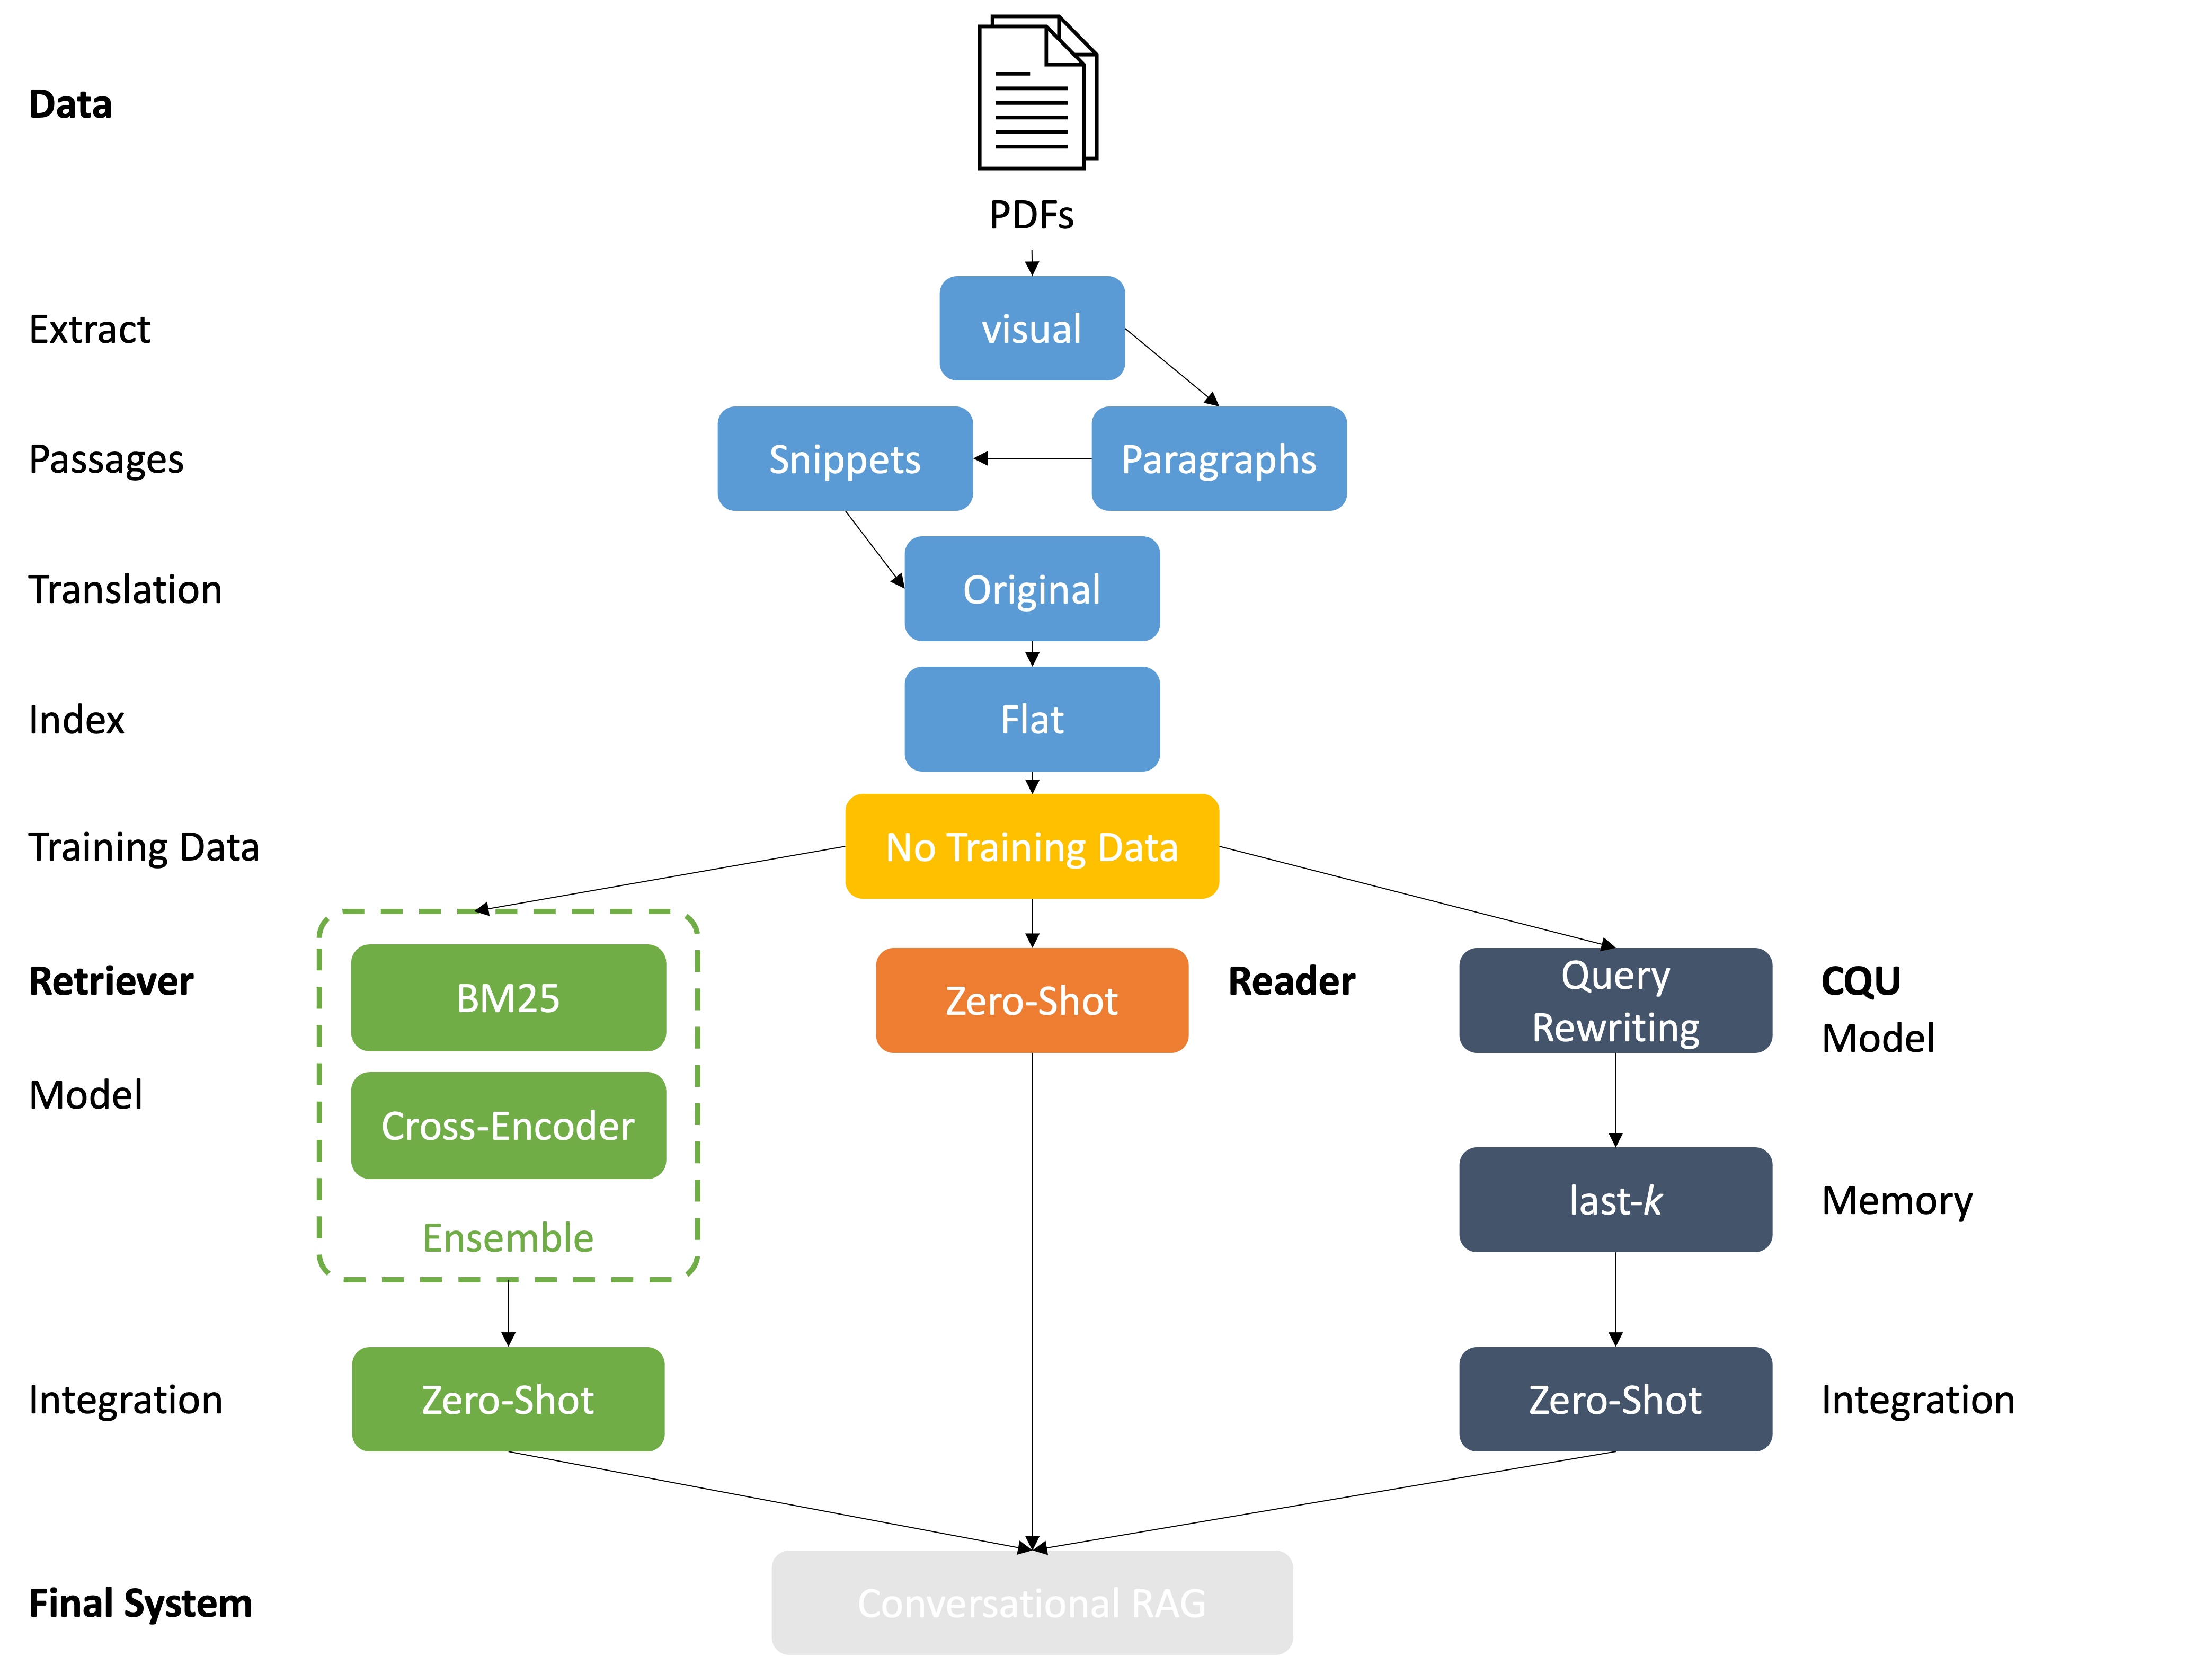
\includegraphics[width=\textwidth]{Grafiken/example_decission_tree.png}
    \caption{Example Implementation Zero-Shot Baseline}
    \label{fig:example-implementation-tree}
\end{figure}

\section{Data Augmentation Implementation}
\label{ref:appendixA-data-augmentation}

\subsection{Examples for Few-Shot Prompt}
\label{ref:appendixA-data-augmentation-few-shot-prompt}

\begin{quote}
    1. Example:\\
        Context: The master's program in Data and Computer Science includes an application area. Annex 3 lists the possible application areas. Upon request, the examination board can also approve a different application area. - Master Data and Computer Science \\
        Question: I study Data and Computerscience. Can I choose application areas that are not listed? \\ \\
    2. Example: \\
        Context: (5) The final failure in a mandatory module leads to the loss of the examination claim. In elective mandatory modules, if provided for in the module handbook, the failure can be compensated for by the successful completion of another elective mandatory module or another performance within the respective module. § 4 Paragraph 2 remains unaffected. - Bachelor Physics \\
        Question: When does the failure of an exam lead to the termination of the study? \\ \\
    3. Example: \\
        Context: (3) The application must be made in writing to the examination board. It is the responsibility of the applicant to provide the necessary information about the performance to be recognized. The burden of proof for the existence of a significant difference in academic achievements lies with Heidelberg University; the obligations of the applicant, especially according to Sentence 1 and Sentence 2, remain unaffected. The burden of proof for the existence of equivalence in non-academic achievements lies with the applicant. - Bachelor Philosophy \\
        Question: What would happen, if I can't provide information on my academic achievements?\\ \\
    4. Example: \\
        Context: The intermediate examination consists of successful participation in the exercises for beginners in the subjects Civil Law, Public Law, and Criminal Law. The partial performances of the exercise (homework and supervisory work under examination conditions) must in principle be performed in the exercise of a semester; § 4 paragraph 5 remains unaffected. - Civil Law\\
        Question: What are the components of the intermediate examination in Civil Law, Public Law, and Criminal Law? \\
\end{quote}

\section{Evaluation}
\label{ref:appendixA-evaluation}

\subsection{Model Configurations}
\label{ref:appendixA-evaluation-model-configurations}

\begin{table}[H]
    \resizebox{\textwidth}{!}{%
    \begin{tabular}{llrrrr}
    \hline
    Application           & Model-Language         & \textit{top k} & \textit{top p} & \textit{temperature} & \textit{repetition penalty} \\ \hline
    \multirow{4}{*}{CQU}  & gpt-3.5-turbo-de       & -*             & 1              & 1                    & 0                           \\
                          & gpt-3.5-turbo-en       & -*             & 1              & 1                    & 0                           \\
                          & leo-hessian-7B-chat-de & 60             & 0.95           & 0.9                  & 1.2                         \\
                          & Llama2-7B-chat-en      & 1              & 0.1            & 0.3                  & 1.4                         \\ \hline
    \multirow{4}{*}{Chat} & gpt-3.5-turbo-de       & -*             & 1              & 1                    & 0                           \\
                          & gpt-3.5-turbo-en       & -*             & 1              & 1                    & 0                           \\
                          & leo-hessian-7B-chat-de & 10             & 0.6            & 0.4                  & 0                           \\
                          & Llama2-7B-chat-en      & 40             & 0.8            & 0.5                  & 1.5                         \\ \hline
    \end{tabular}%
    }
    {\footnotesize * OpenAI does not expose the \textit{top k} parameter for the GPT-3.5-turbo models.}
    \caption{Parameters used for Models in End-to-End Evaluation}
    \label{tab:appendix-parameters-ete}
\end{table}


\subsection{Retriever}
\label{ref:appendixA-evaluation-retriever}

\begin{sidewaystable}
    \centering    
    \begin{tabular}{lrrrrrrrr}
    \toprule
    index & \multicolumn{4}{r}{IndexEnglish} & \multicolumn{4}{r}{IndexGerman} \\
    metric & \multicolumn{2}{r}{HR} & \multicolumn{2}{r}{MRR} & \multicolumn{2}{r}{HR} & \multicolumn{2}{r}{MRR} \\
    retriever & BM25 & DPR & BM25 & DPR & BM25 & DPR & BM25 & DPR \\
    k &  &  &  &  &  &  &  &  \\
    \midrule
    1 & 0.236152 & 0.346251 & 0.236152 & 0.346251 & 0.221038 & 0.235225 & 0.221038 & 0.235225 \\
    3 & 0.347355 & 0.496136 & 0.284705 & 0.412255 & 0.317794 & 0.342329 & 0.263626 & 0.282504 \\
    5 & 0.400344 & 0.560026 & 0.296833 & 0.426853 & 0.360997 & 0.389765 & 0.273503 & 0.293309 \\
    10 & 0.479333 & 0.645523 & 0.307341 & 0.438297 & 0.423759 & 0.459314 & 0.281863 & 0.302535 \\
    15 & 0.530269 & 0.696031 & 0.311357 & 0.442275 & 0.462978 & 0.500956 & 0.284947 & 0.305811 \\
    25 & 0.598848 & 0.760644 & 0.314831 & 0.445564 & 0.511582 & 0.556726 & 0.287416 & 0.308630 \\
    50 & 0.693761 & 0.843895 & 0.317537 & 0.447936 & 0.584736 & 0.637499 & 0.289478 & 0.310920 \\
    100 & 0.769780 & 0.910700 & 0.318649 & 0.448917 & 0.660721 & 0.718856 & 0.290569 & 0.312093 \\
    150 & 0.795991 & 0.933902 & 0.318865 & 0.449109 & 0.698262 & 0.754966 & 0.290878 & 0.312391 \\
    200 & 0.813112 & 0.946265 & 0.318964 & 0.449181 & 0.721834 & 0.777181 & 0.291015 & 0.312520 \\
    300 & 0.836275 & 0.958705 & 0.319060 & 0.449232 & 0.751814 & 0.803585 & 0.291139 & 0.312629 \\
    400 & 0.848770 & 0.966037 & 0.319096 & 0.449253 & 0.770087 & 0.820341 & 0.291192 & 0.312677 \\
    500 & 0.857960 & 0.970819 & 0.319117 & 0.449264 & 0.783486 & 0.832689 & 0.291222 & 0.312705 \\
    1000 & 0.884140 & 0.983089 & 0.319155 & 0.449282 & 0.818224 & 0.864172 & 0.291272 & 0.312751 \\
    \bottomrule
    \end{tabular}
    \caption{Retriever comparison BM25 and DPR over indexEnglish and indexGerman}
\end{sidewaystable}

\begin{sidewaystable}
    \centering    
    \begin{tabular}{lrrrrrrrr}
    \toprule
    index & \multicolumn{4}{r}{translated IndexEnglish} & \multicolumn{4}{r}{translated IndexGerman} \\
    metric & \multicolumn{2}{r}{HR} & \multicolumn{2}{r}{MRR} & \multicolumn{2}{r}{HR} & \multicolumn{2}{r}{MRR} \\
    retriever & BM25 & DPR & BM25 & DPR & BM25 & DPR & BM25 & DPR \\
    k &  &  &  &  &  &  &  &  \\
    \midrule
    1 & 0.183295 & 0.300796 & 0.183295 & 0.300796 & 0.168289 & 0.226307 & 0.168289 & 0.226307 \\
    3 & 0.283473 & 0.439959 & 0.227119 & 0.362059 & 0.255251 & 0.332098 & 0.206333 & 0.272683 \\
    5 & 0.331586 & 0.502232 & 0.238078 & 0.376290 & 0.296455 & 0.379140 & 0.215718 & 0.283417 \\
    10 & 0.402085 & 0.586524 & 0.247408 & 0.387556 & 0.356575 & 0.445857 & 0.223716 & 0.292320 \\
    15 & 0.449383 & 0.638004 & 0.251129 & 0.391613 & 0.394480 & 0.488156 & 0.226698 & 0.295654 \\
    25 & 0.514843 & 0.703348 & 0.254438 & 0.394939 & 0.446412 & 0.543634 & 0.229318 & 0.298465 \\
    50 & 0.610612 & 0.793301 & 0.257162 & 0.397506 & 0.523755 & 0.625181 & 0.231502 & 0.300771 \\
    100 & 0.702672 & 0.874887 & 0.258492 & 0.398697 & 0.606892 & 0.708026 & 0.232692 & 0.301962 \\
    150 & 0.742715 & 0.903959 & 0.258823 & 0.398938 & 0.648592 & 0.747902 & 0.233035 & 0.302293 \\
    200 & 0.768902 & 0.920427 & 0.258974 & 0.399033 & 0.675069 & 0.770949 & 0.233188 & 0.302426 \\
    300 & 0.802740 & 0.938948 & 0.259113 & 0.399109 & 0.709398 & 0.798929 & 0.233329 & 0.302542 \\
    400 & 0.823531 & 0.950183 & 0.259174 & 0.399142 & 0.730504 & 0.815699 & 0.233391 & 0.302590 \\
    500 & 0.840124 & 0.957656 & 0.259211 & 0.399159 & 0.746355 & 0.828033 & 0.233426 & 0.302618 \\
    1000 & 0.884777 & 0.973681 & 0.259276 & 0.399182 & 0.790784 & 0.861399 & 0.233490 & 0.302667 \\
    \bottomrule
    \end{tabular}
    \caption{Retriever comparison BM25 and DPR over translated IndexEnglish and translated IndexGerman}
\end{sidewaystable}

\begin{sidewaystable}
    \begin{tabular}{l*{12}{p{1.32cm}}}
        \toprule
        index & \multicolumn{6}{r}{IndexEnglish} & \multicolumn{6}{r}{IndexGerman} \\
        metric & \multicolumn{3}{r}{HR} & \multicolumn{3}{r}{MRR} & \multicolumn{3}{r}{HR} & \multicolumn{3}{r}{MRR} \\
        retriever & BM25-CE-1000 & BM25-CE-500 & DPR & BM25-CE-1000 & BM25-CE-500 & DPR & BM25-CE-1000 & BM25-CE-500 & DPR & BM25-CE-1000 & BM25-CE-500 & DPR \\
        k &  &  &  &  &  &  &  &  &  &  &  &  \\
        \midrule
        1 & 0.289670 & 0.290665 & 0.346251 & 0.289670 & 0.290665 & 0.346251 & 0.183031 & 0.187395 & 0.235225 & 0.183031 & 0.187395 & 0.235225 \\
        3 & 0.412333 & 0.413632 & 0.496136 & 0.343724 & 0.344858 & 0.412255 & 0.286573 & 0.292441 & 0.342329 & 0.228314 & 0.233467 & 0.282504 \\
        5 & 0.468588 & 0.470151 & 0.560026 & 0.356579 & 0.357755 & 0.426853 & 0.334973 & 0.342475 & 0.389765 & 0.239329 & 0.244864 & 0.293309 \\
        10 & 0.553105 & 0.553665 & 0.645523 & 0.367850 & 0.368904 & 0.438297 & 0.405514 & 0.414301 & 0.459314 & 0.248710 & 0.254398 & 0.302535 \\
        \bottomrule
    \end{tabular}
    \caption{Retriever comparison BM25-CE versions and DPR over IndexEnglish and IndexGerman}
\end{sidewaystable}

\begin{sidewaystable}
    \begin{tabular}{l*{10}{p{1.32cm}}}
        \toprule
        index & \multicolumn{4}{r}{translated IndexEnglish} & \multicolumn{6}{r}{translated IndexGerman} \\
        metric & \multicolumn{2}{r}{HR} & \multicolumn{2}{r}{MRR} & \multicolumn{3}{r}{HR} & \multicolumn{3}{r}{MRR} \\
        retriever & BM25-CE-500 & DPR & BM25-CE-500 & DPR & BM25-CE-1000 & BM25-CE-500 & DPR & BM25-CE-1000 & BM25-CE-500 & DPR \\
        k &  &  &  &  &  &  &  &  &  &  \\
        \midrule
        1 & 0.226215 & 0.300796 & 0.226215 & 0.300796 & 0.210515 & 0.211157 & 0.226307 & 0.210515 & 0.211157 & 0.226307 \\
        3 & 0.357346 & 0.439959 & 0.283679 & 0.362059 & NaN & 0.315852 & 0.332098 & NaN & 0.257302 & 0.272683 \\
        5 & 0.418429 & 0.502232 & 0.297588 & 0.376290 & 0.363084 & 0.363435 & 0.379140 & 0.267510 & 0.268156 & 0.283417 \\
        10 & 0.500264 & 0.586524 & 0.308518 & 0.387556 & 0.430064 & 0.429218 & 0.445857 & 0.276427 & 0.276925 & 0.292320 \\
        \bottomrule
    \end{tabular}
    \caption{Retriever comparison BM25-CE versions and DPR over translated IndexEnglish and translated IndexGerman}
\end{sidewaystable}
